\documentclass[12pt]{exam}
\usepackage[utf8]{inputenc}

\usepackage{amsmath,amstext,amsthm,amssymb,amsxtra}
\usepackage[top=1.5in, bottom=1.5in, left=1.25in, right=1.25in]{geometry}
\usepackage{txfonts}
\usepackage[T1]{fontenc}
\usepackage{lmodern}
\renewcommand*\familydefault{\sfdefault}
\usepackage{euler}
\usepackage{pdfsync}
\usepackage{multicol}
\newcommand{\ci}[1]{_{ {}_{\scriptstyle #1}}}
\usepackage{graphicx}
\graphicspath{ {images/} }
\usepackage{tikz}

\newcommand{\norm}[1]{\ensuremath{\left\|#1\right\|}}
\newcommand{\abs}[1]{\ensuremath{\left\vert#1\right\vert}}
\newcommand{\ip}[2]{\ensuremath{\left\langle#1,#2\right\rangle}}
\newcommand{\p}{\ensuremath{\partial}}
\newcommand{\pr}{\mathcal{P}}

\newcommand{\pbar}{\ensuremath{\bar{\partial}}}
\newcommand{\db}{\overline\partial}
\newcommand{\D}{\mathbb{D}}
\newcommand{\B}{\mathbb{B}}
\newcommand{\Sp}{\mathbb{S}}
\newcommand{\T}{\mathbb{T}}
\newcommand{\R}{\mathbb{R}}
\newcommand{\Z}{\mathbb{Z}}
\newcommand{\C}{\mathbb{C}}
\newcommand{\N}{\mathbb{N}}
\newcommand{\Q}{\mathbb{Q}}
\newcommand{\mQ}{\mathcal{Q}}
\newcommand{\mS}{\mathcal{S}}
\newcommand{\scrH}{\mathcal{H}}
\newcommand{\scrL}{\mathcal{L}}
\newcommand{\td}{\widetilde\Delta}
\newcommand{\pw}{\text{PW}}
\newcommand{\esup}{\text{ess.sup}}
\newcommand{\Tn}{\mathcal{T}_n}
\newcommand{\Bn}{\mathbb{B}_n}
\newcommand{\rt}{\mathcal{O}}
\newcommand{\avg}[1]{\langle #1 \rangle}
\newcommand{\one}{\mathbbm{1}}
\newcommand{\eps}{\varepsilon}
\newcommand{\grad}{\nabla}

\newcommand{\La}{\langle }
\newcommand{\Ra}{\rangle }
\newcommand{\rk}{\operatorname{rk}}
\newcommand{\card}{\operatorname{card}}
\newcommand{\ran}{\operatorname{Ran}}
\newcommand{\osc}{\operatorname{OSC}}
\newcommand{\im}{\operatorname{Im}}
\newcommand{\re}{\operatorname{Re}}
\newcommand{\tr}{\operatorname{tr}}
\newcommand{\vf}{\varphi}
\newcommand{\f}[2]{\ensuremath{\frac{#1}{#2}}}

\newcommand{\kzp}{k_z^{(p,\alpha)}}
\newcommand{\klp}{k_{\lambda_i}^{(p,\alpha)}}
\newcommand{\TTp}{\mathcal{T}_p}
\newcommand{\m}[1]{\mathcal{#1}}
\newcommand{\md}{\mathcal{D}}
\newcommand{\qan}{\abs{Q}^{\alpha/n}}
\newcommand{\sbump}[2]{[[ #1,#2 ]]}
\newcommand{\mbump}[2]{\lceil #1,#2 \rceil}
\newcommand{\cbump}[2]{\lfloor #1,#2 \rfloor}

\newcommand{\class}{Math 629 Spring 26}
\newcommand{\term}{Fall 24}
\newcommand{\examnum}{Homework \hwnum}
\newcommand{\examdate}{\duedate}
\newcommand{\timelimit}{75 Minutes}
\newcommand{\vc}[3]{\langle #1,#2,#3\rangle}
\newcommand*{\vv}[1]{\vec{\mkern0mu#1}}
\newcommand{\bv}[1]{\boldsymbol{#1}}
\newcommand{\hide}[1]{}
\newcommand{\uvec}[1]{\boldsymbol{\hat{\textbf{#1}}}}
\newcommand{\vex}[1]{\boldsymbol{{\textbf{#1}}}}

\pagestyle{head}
\firstpageheader{}{}{}
\runningheader{\class}{\examnum\ - Page \thepage\ of \numpages}{\examdate}
\runningheadrule

\makeatletter
\renewcommand*\env@matrix[1][*\c@MaxMatrixCols c]{%
  \hskip -\arraycolsep
  \let\@ifnextchar\new@ifnextchar
  \array{#1}}
\makeatother

%\printanswers
\begin{document}

\noindent
\begin{tabular*}{\textwidth}{l @{\extracolsep{\fill}} r @{\extracolsep{6pt}} l}
\textbf{\class} & \textbf{Name: Mengxiang Jiang}\\
\end{tabular*}\\
\rule[2ex]{\textwidth}{2pt}

\newcommand{\duedate}{04/13/2026 at 11:59pm}
\newcommand\hwnum{12}

Turn this assignment in on Gradescope. All work must be neat and legible. Turn in 
a ``final draft''. There should be nothing scratched out and your work should flow
generally from left to right and top to bottom.

\begin{questions}


\question
Show that $\sin x$ is continuous at all values of $x$ (Hint: $\sin(x+\alpha) - \sin x = 2\sin(\frac{1}{2}\alpha) \cos(x + \frac{1}{2}\alpha)$).
\\\\
Using the identity in the hint, we take the absolute values:
\[
  |\sin(x+\alpha) - \sin x| = 2\left|\sin\left(\frac{1}{2}\alpha\right)\right| \cdot \left|\cos\left(x + \frac{1}{2}\alpha\right)\right|.
\]
Since $|\cos x| \leq 1$ for all $x$, and $|\sin(x)| \leq |x|$ for all $x$, we have:
\[
  |\sin(x+\alpha) - \sin x| \leq 2\left|\sin\left(\frac{1}{2}\alpha\right)\right| \leq 2\left|\frac{1}{2}\alpha\right| = |\alpha|.
\]
Thus, for any $\epsilon > 0$, if we choose $\delta = \epsilon$, then whenever $|\alpha| < \delta$, we have:
\[
  |\sin(x+\alpha) - \sin x| < \epsilon.
\]
This shows that $\sin x$ is continuous at all values of $x$.
\newpage 
\question
What is $\lim_{a\to 0}\frac{\sin a}{a}$? Assuming that $\cos$ is continuous, use the above to find the derivative 
of $\sin x$. 
\\\\
I remember getting points taken off an exam for using L'Hopital's for this, so I learned to do it through geometry. Consider the diagram below with three areas:
\begin{figure}[h!]
\centering
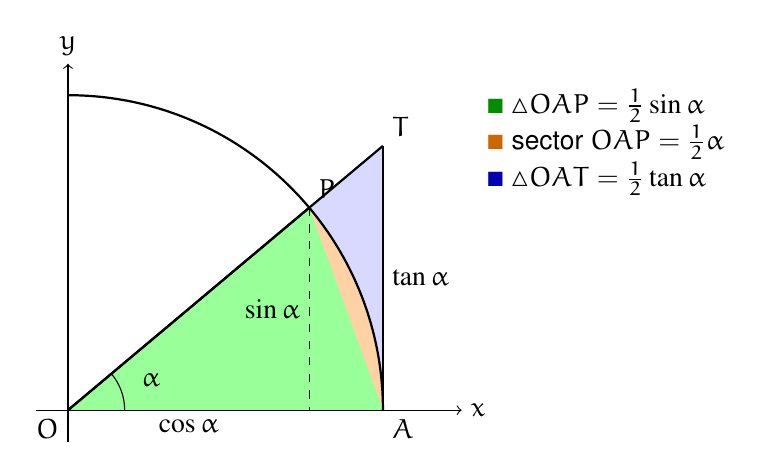
\begin{tikzpicture}[scale=4]
    % Angle for illustration
    \def\a{40}

    % Right triangle OAT (outer): vertices O, A=(1,0), T=(1, tan a)
    \fill[blue!15]
        (0,0) -- (1,0) -- (1,{tan(\a)}) -- cycle;

    % Circular sector OAP: bounded by OA, arc from A to P, and PO
    \fill[orange!35]
        (0,0) -- (1,0) arc[start angle=0, end angle=\a, radius=1] -- cycle;

    % Inner triangle OAP: vertices O, A=(1,0), P=(cos a, sin a)
    \fill[green!40]
        (0,0) -- (1,0) -- ({cos(\a)},{sin(\a)}) -- cycle;

    % Unit circle (arc only, for reference)
    \draw[thick] (1,0) arc[start angle=0, end angle=90, radius=1];

    % Axes
    \draw[->] (-0.1,0) -- (1.25,0) node[right] {$x$};
    \draw[->] (0,-0.1) -- (0,1.1) node[above] {$y$};

    % Radii and tangent segment
    \draw[thick] (0,0) -- ({cos(\a)},{sin(\a)});
    \draw[thick] (0,0) -- (1,{tan(\a)});
    \draw[thick] (1,0) -- (1,{tan(\a)});

    % Drop perpendicular from P to x-axis (to show sin a)
    \draw[dashed] ({cos(\a)},{sin(\a)}) -- ({cos(\a)},0);

    % Angle arc near origin
    \draw (0.18,0) arc[start angle=0, end angle=\a, radius=0.18];
    \node at ({0.28*cos(\a/2)},{0.28*sin(\a/2)}) {$\alpha$};

    % Point labels
    \node[below left]  at (0,0)                         {$O$};
    \node[below right] at (1,0)                         {$A$};
    \node[above right] at (1,{tan(\a)})                 {$T$};
    \node[above right] at ({cos(\a)},{sin(\a)})         {$P$};

    % Segment labels
    \node[right] at (1,{0.5*tan(\a)})                   {$\tan\alpha$};
    \node[left]  at ({cos(\a)},{0.5*sin(\a)})           {$\sin\alpha$};
    \node[below] at ({0.5*cos(\a)},0)                   {$\cos\alpha$};

    % Area legend
    \node[align=left, anchor=west] at (1.3,0.85)
        {\textcolor{green!55!black}{$\blacksquare$} $\triangle OAP = \tfrac{1}{2}\sin\alpha$ \\
         \textcolor{orange!80!black}{$\blacksquare$} sector $OAP = \tfrac{1}{2}\alpha$ \\
         \textcolor{blue!70!black}{$\blacksquare$} $\triangle OAT = \tfrac{1}{2}\tan\alpha$};
\end{tikzpicture}
\end{figure}
\linebreak
From the diagram, we have the following inequalities:
\[
  \frac{1}{2}\sin a \leq \frac{1}{2}a \leq \frac{1}{2}\tan a.
\]
Dividing through by $\frac{1}{2}\sin a$ and inverting the inequalities, we get:
\[
 \cos a \leq \frac{\sin a}{a} \leq 1.
\]
Taking the limit as $a \to 0$, we have $\lim_{a \to 0} \cos a = 1$ and $\lim_{a \to 0} 1 = 1$. By the squeeze theorem, we conclude that $\lim_{a \to 0} \frac{\sin a}{a} = 1$.
\\\\
To find the derivative of $\sin x$, we use the definition of the derivative, the identity from the first question, and the limit we just found:
\begin{align*}
  \frac{d}{dx} \sin x &= \lim_{h \to 0} \frac{\sin(x+h) - \sin x}{h} \\
  &= \lim_{h \to 0} \frac{2\sin\left(\frac{1}{2}h\right) \cos\left(x + \frac{1}{2}h\right)}{h} \\
  &= \lim_{h \to 0} \cos\left(x + \frac{1}{2}h\right) \cdot \lim_{h \to 0} \frac{\sin\left(\frac{1}{2}h\right)}{\frac{1}{2}h} \\
  &= \cos(x) \cdot 1 = \cos x.
\end{align*}
\newpage 
\question
If $A < \frac{a_k}{b_k}<B$ for $k=1, \ldots, N$ then 
$A < \frac{\sum_{k=1}^{N}a_k}{\sum_{k=1}^{N}b_k} < B$.
\\\\
From $A < \frac{a_k}{b_k} < B$, we can multiply through by $b_k$ to get:
\[
  Ab_k < a_k < Bb_k.
\]
Summing over $k$ from 1 to $N$, we obtain:
\[
  A\sum_{k=1}^{N} b_k < \sum_{k=1}^{N} a_k < B\sum_{k=1}^{N} b_k.
\]
Dividing through by $\sum_{k=1}^{N} b_k$, we get:
\[
  A < \frac{\sum_{k=1}^{N} a_k}{\sum_{k=1}^{N} b_k} < B.
\]
\end{questions}
\end{document}